\documentclass[review, times]{elsarticle}

%%%%%%%%%%%%%%   Preample  %%%%%%%%%%%%%%%%%%
%% for comment (texts in between \begin{comment} and \end{comment} will be ignored)
\usepackage{comment} 

%% The amssymb package provides various useful mathematical symbols
\usepackage{amssymb}
%% The amsthm package provides extended theorem environments
\usepackage{amsthm}

%% for celcius symbol
\usepackage{textcomp}

%% for units
\usepackage{siunitx}

%% multirow
\usepackage{multirow}

%% The lineno packages adds line numbers. Start line numbering with
%% \begin{linenumbers},  end it with \end{linenumbers}. Or switch it on
%% for the whole article with \linenumbers.
\usepackage{lineno}
\modulolinenumbers[5]
%\linenumbers

\usepackage{hyperref}

%% package for subfigure environment
\usepackage{subcaption}

%% package for type Greek letters without entering into math-mode
\usepackage{textgreek}

%% package for large picture in two-colume
\usepackage{dblfloatfix}
\usepackage{fixltx2e}
\usepackage{float}
%\usepackage{placeins}
\usepackage{subcaption}

%% only jpg pdf eps are allowed, tiff format are not allowed in latex
%% eps in principle can't be compiled by pdflatex, pdf not compiled by latex, but Kile can do some intermedate conversion to allow this happen.
\DeclareGraphicsExtensions{.pdf, .eps, .jpg}
%%opening
\journal{NIMA}

\begin{document}

%%%%%%%%%%%%%% Front Matter %%%%%%%%%%%%%%%%%%
\begin{frontmatter}

\title{A versatile PMT test bench and its application in the DAMPE-PSD}
%%\title{Title with footnote\tnoteref{t1}}
%%\tnotetext[t1]{FootNote for title}

\author[imp,lzu,ucas]{Yong Zhou}
%\ead{yong@impcas.ac.cn}

\author[imp]{Yuhong Yu}
%%\ead{yuyuhong@impcas.ac.cn}

\author[imp]{Zhiyu Sun\corref{corresponding_author}}
\cortext[corresponding_author]{Corresponding author}
\ead{sunzhy@impcas.ac.cn}

\author[imp]{Yongjie Zhang}
\author[imp]{Fang Fang}
\author[imp]{Junling Chen}

\author[lzu]{Bitao Hu}
%% Additional Author information %%
%%\author[ano]{Anonymous\fnref{fn1}}
%%\ead{anonymous@anonymous.cn}
%%\fntext[fn1]{FootNote for Anonymous author}

\address[imp]{Institute of Modern Physicas, Chinese Academy of Sciences,  509 Nanchang Road,  Lanzhou,  730000,  P.R.China}
\address[lzu]{School of Nuclear Science and Technology,  Lanzhou University,  222 South Tianshui Road,  Lanzhou,  730000,  P.R.China}
\address[ucas]{Graduate University of the Chinese Academy of Sciences,  19A Yuquan Road,  Beijing,  100049,  P.R.China}
%%\address[ano]{Anonymous Address of Anonymous author}

%%
\begin{abstract}

A versatile test bench, dedicated for massive PMT characterization, is developped at the Institute of Modern Physics, Chinese Academy of Sciences.
The test bench is suitable for reuse in different applications and incorporates the cathode surface scanning as its intrinsic capability.
Initial application of the test bench in the Plastic Scintillator Strip Detector of DArk Matter Paricle Explorer is successfull and a total of 570 Hamamastu R4443 Mod2 tubes have been charaterized.
Implementation details of the test bench is described in this article.
Major results and performance of the test bench during this application are also reported. 
\end{abstract}

%%
\begin{keyword}
PMT
\sep test bench
\sep DAMPE-PSD

%% PACS codes here,  in the form: \PACS code \sep codes

%% MSC codes here,  in the form: \MSC code \sep code
%% or \MSC[2008] code \sep code (2000 is the default)

\end{keyword}

\end{frontmatter}
\linenumbers
%%%%%%%%%%%%%%%%  Introduction  %%%%%%%%%%%%%%%%%%%%%%%
\section{Introduction}
\label{sec:introduction}

Since invented about 80 years ago, Photomultiplier tubes( PMTs) have been widely used as photosensors in nuclear and particle physics experiments due to the high sensitivity, fast time response and other benefits they have.
Today, large experiments may contain thousands or even more PMTs.
To optimize the detector's performance as a whole, it's important to study the characteristics of each PMT before they are put into usage. 
Manufacturers will always provide some information about the PMTs they offered, but this only gives a rough indication of the performance because their test procedures are quite different from the usage of PMT in real cases.
On the other hand, experiments may have special requirements for some characteristics of PMTs, which the manufacturers can not provide. 
Thus characterization of PMTs in the laboratoy is mandatory in large experiments.

Testing a large number of PMTs in limited time is a tough job, and usually a dedicated test bench is constructed to facilitate this work~\cite{barnhill_testing_2008,akgun_complete_2005,adragna_pmt-block_2006}.
Setting up a system like this is none trivial work, which demands considerable investment of time and effort.
On the other hand, testing of PMTs is a commonly encountered procedure and many components of the testing configuration can be shared among different applications.
%Thus, it is desirable that the same test bench, with minimum configuration changes, can be reused in different applications. 

In this paper, a versatile test bench dedicated for PMT characterization is reported.
The test bench is designed to be a standard laboratoy equipment for fast PMT characterization for several experiments prepared and planned at the Institute of Modern Physics(IMP), Chinese Academy of Sciences.
To accommodate the various requirements of different experiments, the test bench has adoptted a modular design pattern both in the hardware and the associated software platform.
This makes the migration from one testing configuration to another light-weight and time-saving.
Detailed description can be found in Sec.\ref{sec:description}.

The first user of this test bench is the Plastic Scintillator Detector(PSD), a key component of the DArk Matter Paricle Explorer(DAMPE)~\cite{Chang_Jin_dampe} which is a statellite-borne exeperiment. 
PSD is a large-area plastic scintillator array which will work for high energy e/$\gamma$ discrimination as well as charge measurement up to Z=20 by measuring the energy deposited.
PSD will use 164 PMTs for readout, and the test work for these PMTs using this test bench is very successfull. 
Some of the test results are shown in Sec.\ref{sec:application}.

%%%%%%%%%%%%%%%% Main Text Body %%%%%%%%%%%%%%%%%%%%%%%
\section{Description of the test bench}
\label{sec:description}

\begin{figure*}
 \centering
 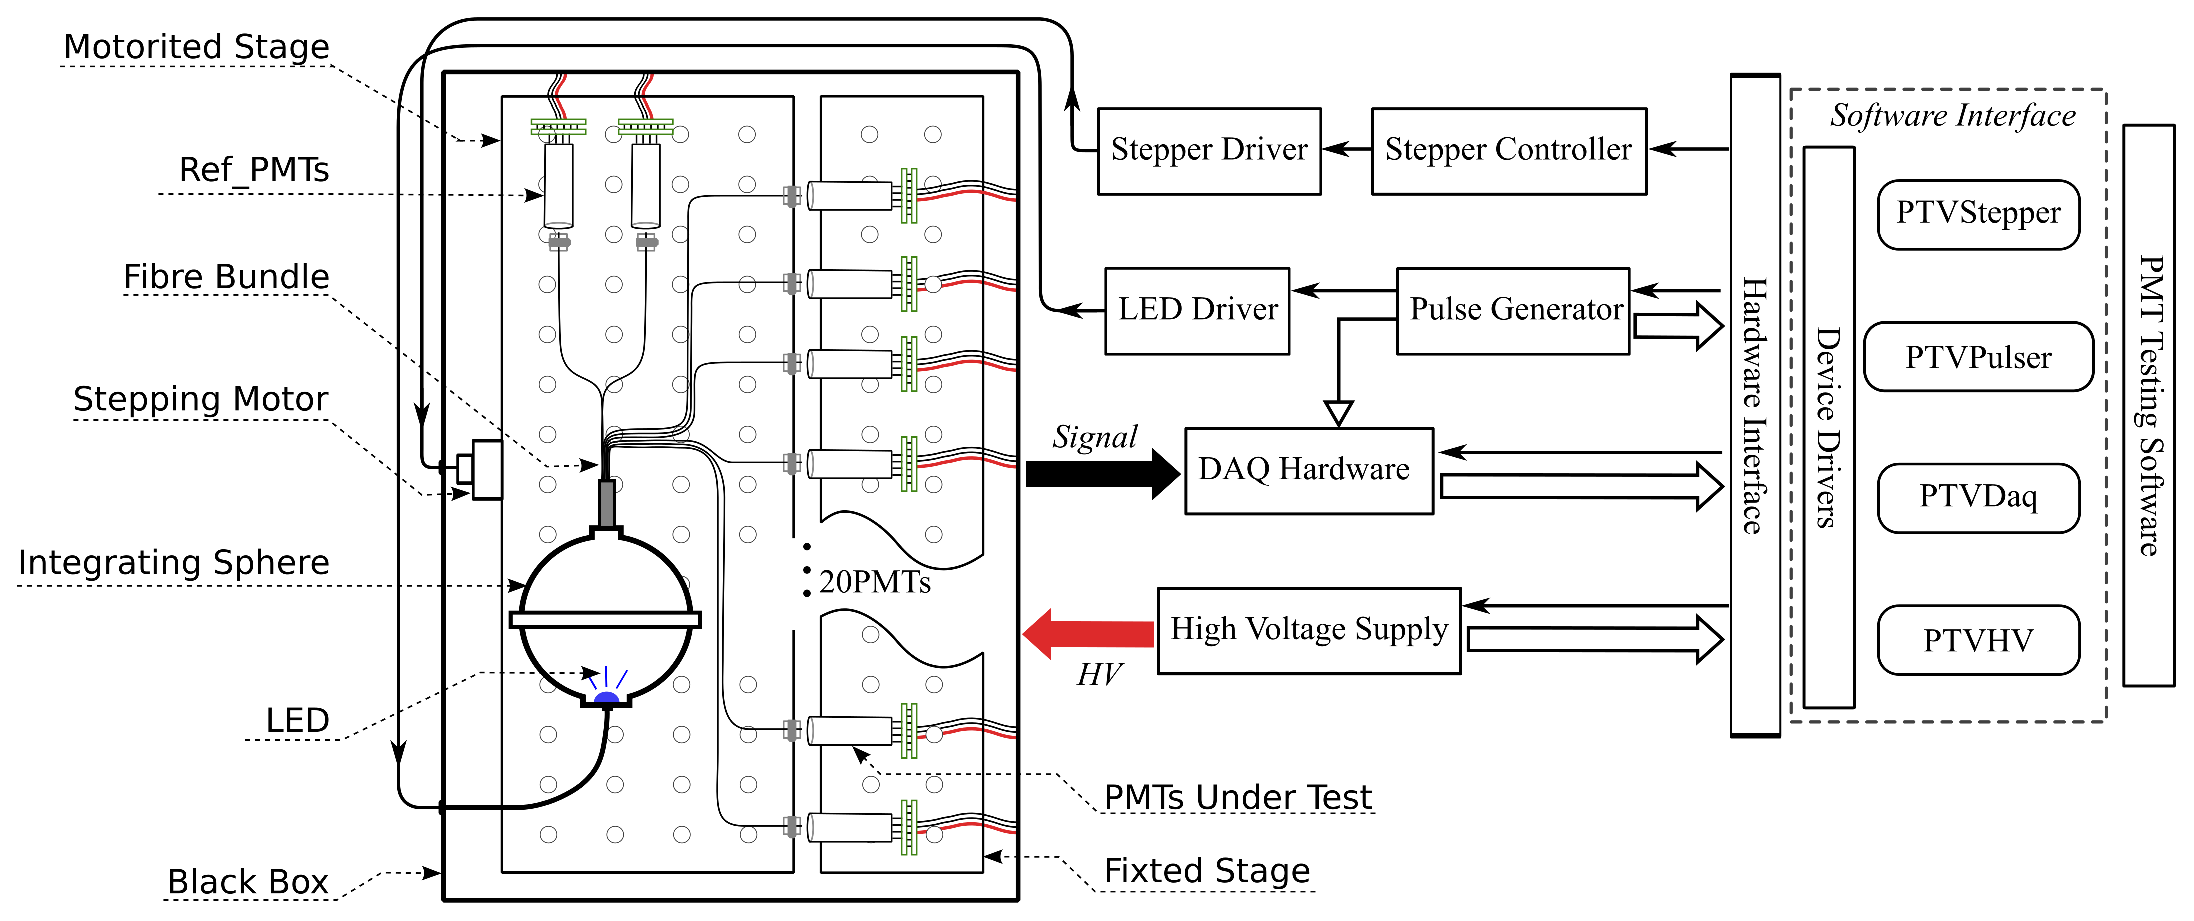
\includegraphics[width=140mm]{testbench_overview}
\caption{Schematic diagram of the PMT test bench system.}
\label{fig:testbench_overveiw}
\end{figure*}

As a massive PMT test bench, some aspects need to be considered in the design:
\begin{itemize}
 \item \textit{Large capacity}: This is the primary driving force for developping a test bench dedicated for massive PMT characterization.
 Testing multiple tubes simultaneously can increase the efficiency and save time tremendously, and this is a critical factor in projects involving large number of PMTs. 
 On the other hand, testing too many tubes at the same time will make the system very complicated and difficult to operate. 
 So we need to make a trade-off between efficiency and complexity.
 \item \textit{Automation}: A single test run for PMT characterization ususally takes several hours, during which most operations are trivial jobs like changing voltage, changing light intensity and so on.
 Manual operations are inefficient and unreliable in such a long period.
 Computer controllable hardwares should be used whenever possible and corresponding software should be developped to automate these trivial operations.
 Manual intervention is only expected in the beginning when mounting PMTs and configuring the software and in the end when unmounting PMTs and assessing testing result. 
 \item \textit{Versatility}: The test bench is not designed for a specific project only.
 We should consider as many potential cases as possible, and appropriate hardwares should be set up in the first place.
 For example, the photocathode scanning capability is desirable in some use cases where many scintillators are coupled to a single PMT~\cite{tof_pet}. 
 \item \textit{Flexibility}: As a by product of versatiltiy, flexibility is needed both in terms of hardware and software.
 The hardware platform should be extensible and allow complex testing configurations.
 The software should accommodate any changes in the hardware easily, while keeping the high level functionality unchanged and portable. 
\end{itemize}

A schematic diagram of the final design is shown in Fig.\ref{fig:testbench_overveiw}, and up to 25 PMTs can be tested simultaneously.
Light pulses are distributed to each tube through an integrating sphere and a fiber bundle, which are mounted on a three-dimensional motorized stage.
PMTs under test will be mounted on a separate fixed stage, thus allowing position scanning of all tubes simultaneously.
There also has 2 PMTs fixed on the motorized stage, serving as a reference to monitor the stability of the light source as well as the performance of the whole system.
Both stages are housed in a light-tight container made of aluminium alloy, with a dimension of $176cm\times100cm\times78cm$.
The container is painted black inside and the lid can be removed for operations such as tube mounting.
Light-tight feedthroughs are left in the side plate of the container for cable routing to the outside.

Auxiliary equipments of the test bench are placed outside the light-tight container.
They can be grouped under four controlling devices, motion controller, pulse generator, high voltage supply and data acquisition system(DAQ), according to the functions they provide.
Among them, pulse generator is used to output trigger pulse to the LED driver as well as to the DAQ simultaneously.

These four kinds of controlling devices are regarded as the essential parts of the test bench as they are needed in every basic PMT characterization.
However, different hardwares may be preferred in different applications.
The motion controller and the pulse generator are tightly coupled to the test bench, so the same hardware can be shared for nearly all the use cases the bench may work for. 
On the other hand, DAQ and the high voltage supply system have more closer relation to the PMTs under test, so they are expected to be replaced frequently. 
Originally, we equiped a CAEN SY1527LC~\cite{sy1527lc} as high voltage supply and a universal CAMAC DAQ system with CC-USB crate controller~\cite{cc_usb}.

The control of all these equipments are integrated into a single software. 
The changing of hardware is handled smoothly in the software design and automation is realized in every aspect of the test bench.

The whole test bench system is sitted in a cleanroom at IMP, and the room temperature is keeped to be 22\textpm~2\textcelsius~all the time.
In the following sections, some key components of the test bench will be described in detail.

%\begin{comment}
\begin{figure}
 \centering
 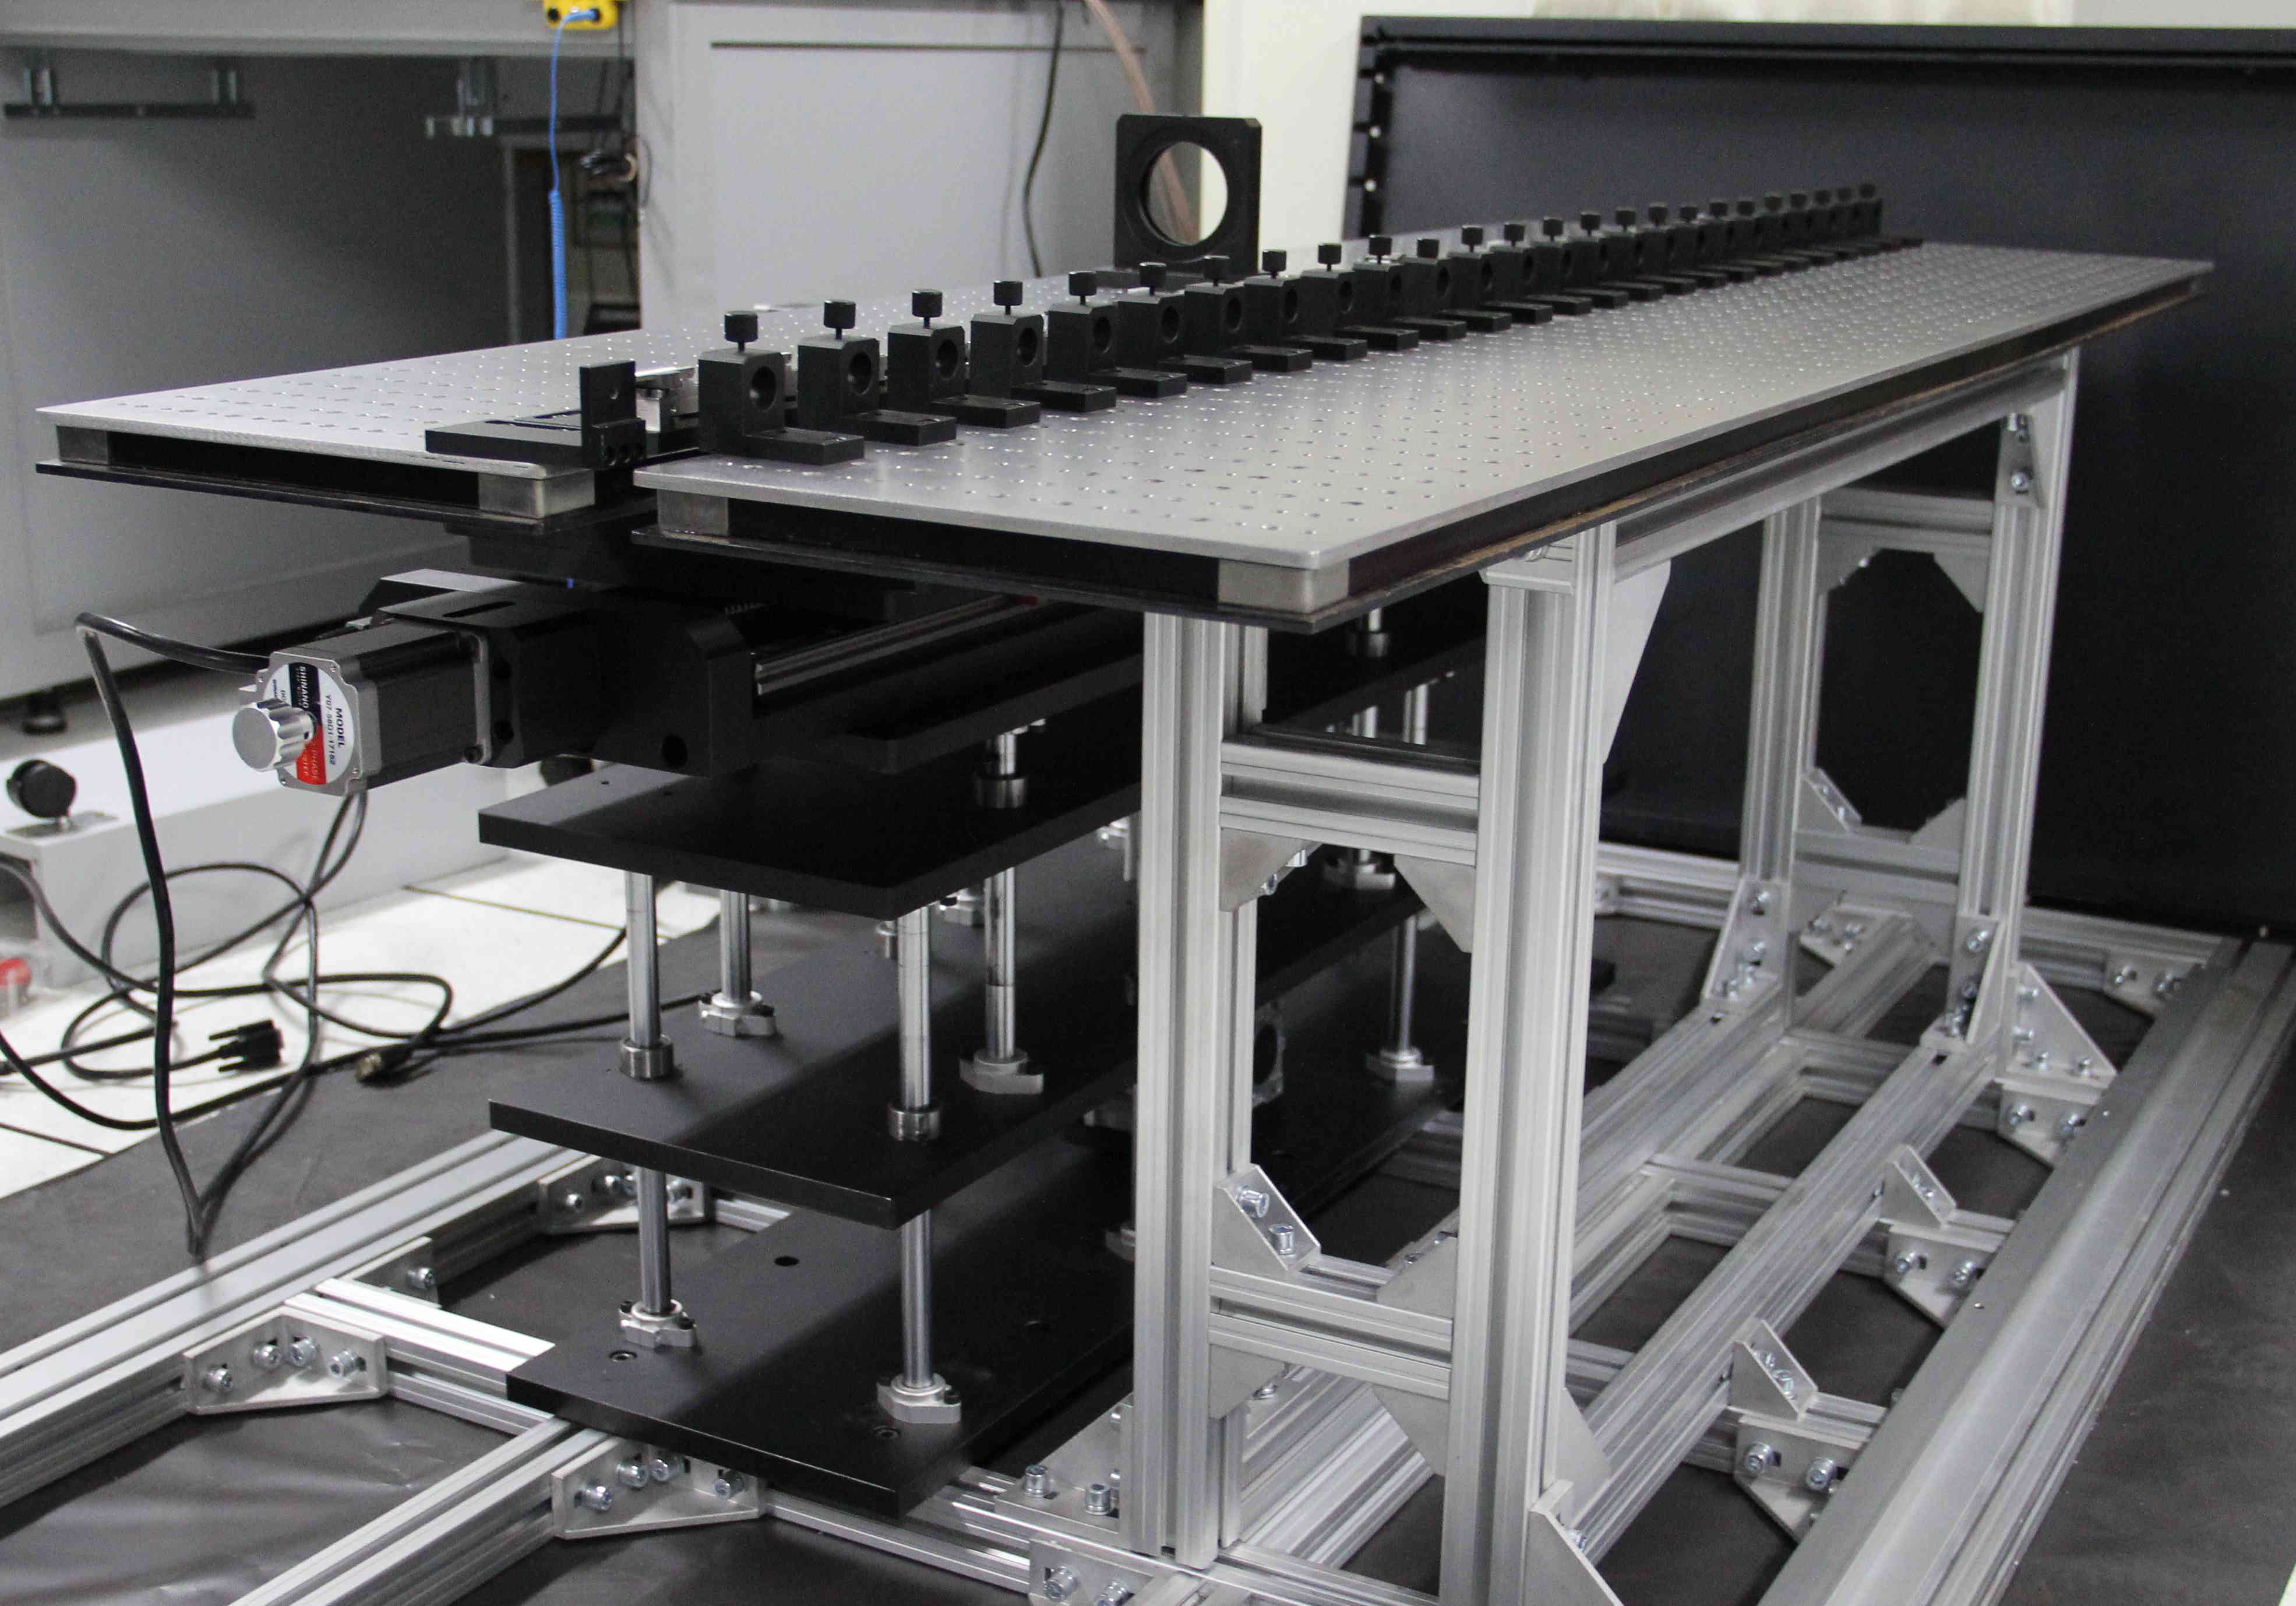
\includegraphics[width=90mm]{stage1_crop}
\caption{Motorized and fixed stages before assembly.
Fixtures for integrationg sphere, fibres and PMTs can be seen on top of them.}
\label{fig:stages}
\end{figure} 
%\end{comment}

\subsection{Motorized and Fixed Stages}
\label{sec:stages}

The motorized and fixed stages are the main body of the test bench.
All other objects inside the light-tight box will be mounted on the top of them.
In particular, customized fixtures for fibres, tubes and integration sphere have been designed for convenient and accurate poistioning.

Both of the stages are covered with an $1560mm\times250mm$ optical breadboard, as shown in Fig.\ref{fig:stages}.
These breadboards are made of \SI{2.5}{cm} thick stainless steel, providing substantial resistance to deformation in the application. 
And the grid pattern of tapped holes on their surface facilitate mounting/unmounting operations as well as provide extra flexibility in the testing configuration.

The load capacity of the motorized stage is \SI{30}{\kilo\gram} and it can do a 3D motion with the help of three stepping motors, which have a minimum step of \SI{1.56}{\micro\meter}.
The stage can move up to \SI{60}{\milli\meter} horizontally and \SI{70}{\milli\meter} vertically, and it's enough to cover any PMTs less than 2 inches, which are mostly used.
The stage can also move along the third direction for $15mm$, and this is to control the gap between the fiber and the window of the tub as well as to protect the fibers while mounting/unmounting the tubes.
All the stepping motors are controlled by one motion controller MPC07SP from Leetro~\cite{leetro}, which also provides a PCI interface for remote control.

\subsection{Light Source}
\label{sec:light_source}

A fast response blue LED(\SI{3}{\watt}, \SIrange{465}{485}{\nano\meter}) is adoptted as the light source of the test bench. 
This kind of LED has been used previously in the monitoring and calibration system of Neutron Wall Detector at IMP~\cite{yuyuhong_led} and proved to be suitable for massive light distribution. 
By coupling to a \SI{5}{\centi\meter} diameter integrating sphere~\cite{integrating_sphere}, which is painted interiorly with highly reflective material($\approx$\SI{98}{\percent} at \SI{400}{\nano\meter}), the LED is converted into a uniform light source.
The LED is fixed on a special designed base using thermally conductive silicone rubber and then coupled to the sphere directly, making the whole sphere as its heat sink.

To drive the LED, we adopted an arbitrary/function generator, the Tektronix AFG3252~\cite{afg3252}. 
AFG3252 can adjust all the pulse parameters, such as width, leading/trailing edge time and amplitude, in a wide range with high precison. 
This is a critical feature for a test bench with an objective of versatiltiy, as diverse requirements for the light source exist in different applications. 
Besides the LED driving pulse, AFG3252 can also output a synchronized pulse as the trigger signal to DAQ system, which will symplify the DAQ configuration in most cases. 
AFG3252 also possesses a rich set of hardware interfaces for remote control.
All these features make it an effective replacement of a dedicated LED driver. 

%Before usage, the relations between the light output of the LED and the setting parameters of AFG3252 are studied carefully. 
Before usage, the uniformity of the light source has been checked by using the same optical fiber to scan the output port surface of the integrating sphere. 
The fiber was coupled to a PMT to measure the light intensity, and the result is shown in Fig.\ref{fig:uniformity_integratingsphere}. 
An uniformity within \textpm\SI{0.5}{\percent} has been reached, and this makes the coupling between the light source and the fiber bundle much easier and additional calibration for the spatial effect of the light source is not needed. 

\begin{figure}
 \centering
 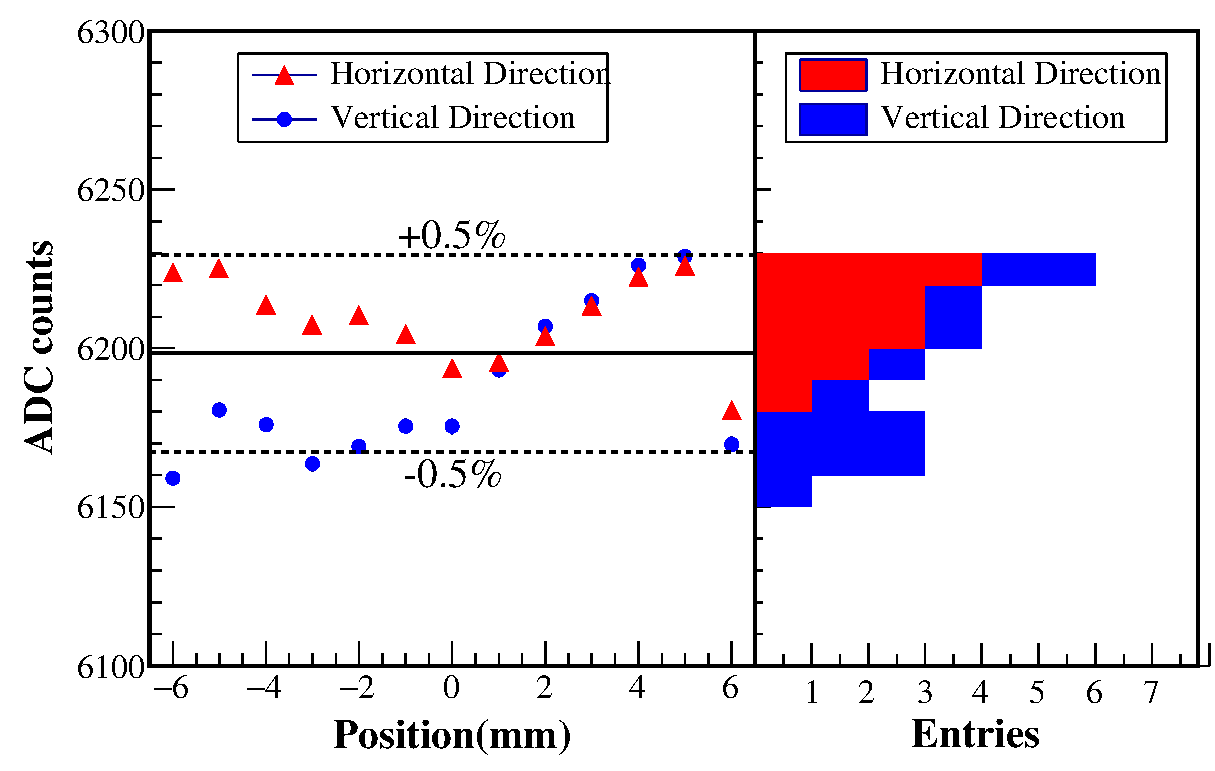
\includegraphics[width=90mm]{uniformity_integratingsphere}
\caption{Spatial uniformity of the integrating sphere.
The output port has a diameter of \SI{14}{\milli\meter}.
Central \SI{12}{\milli\meter} is scanned both in the horizontal and verical direction with a step of \SI{1}{\milli\meter}}
\label{fig:uniformity_integratingsphere}
\end{figure} 

\subsection{Fiber Bundle}
\label{sec:fiber_bundle}

A bundle of 35(25 for test channels, 2 for reference channels and 8 spares) plastic clad silica fibers~\cite{optical_fibre} is utilized to distribute light to each PMT.
Each fiber is \SI{1.5}{\meter} long and has a \SI{400}{\micro\meter} diameter core with a \SI{75}{\micro\meter} thick cladding, and the numerical aperture(NA) is 0.37.
The relatively large core and NA make the fibre an efficient light extracter of integrating sphere output. 

\begin{figure}
 \centering
 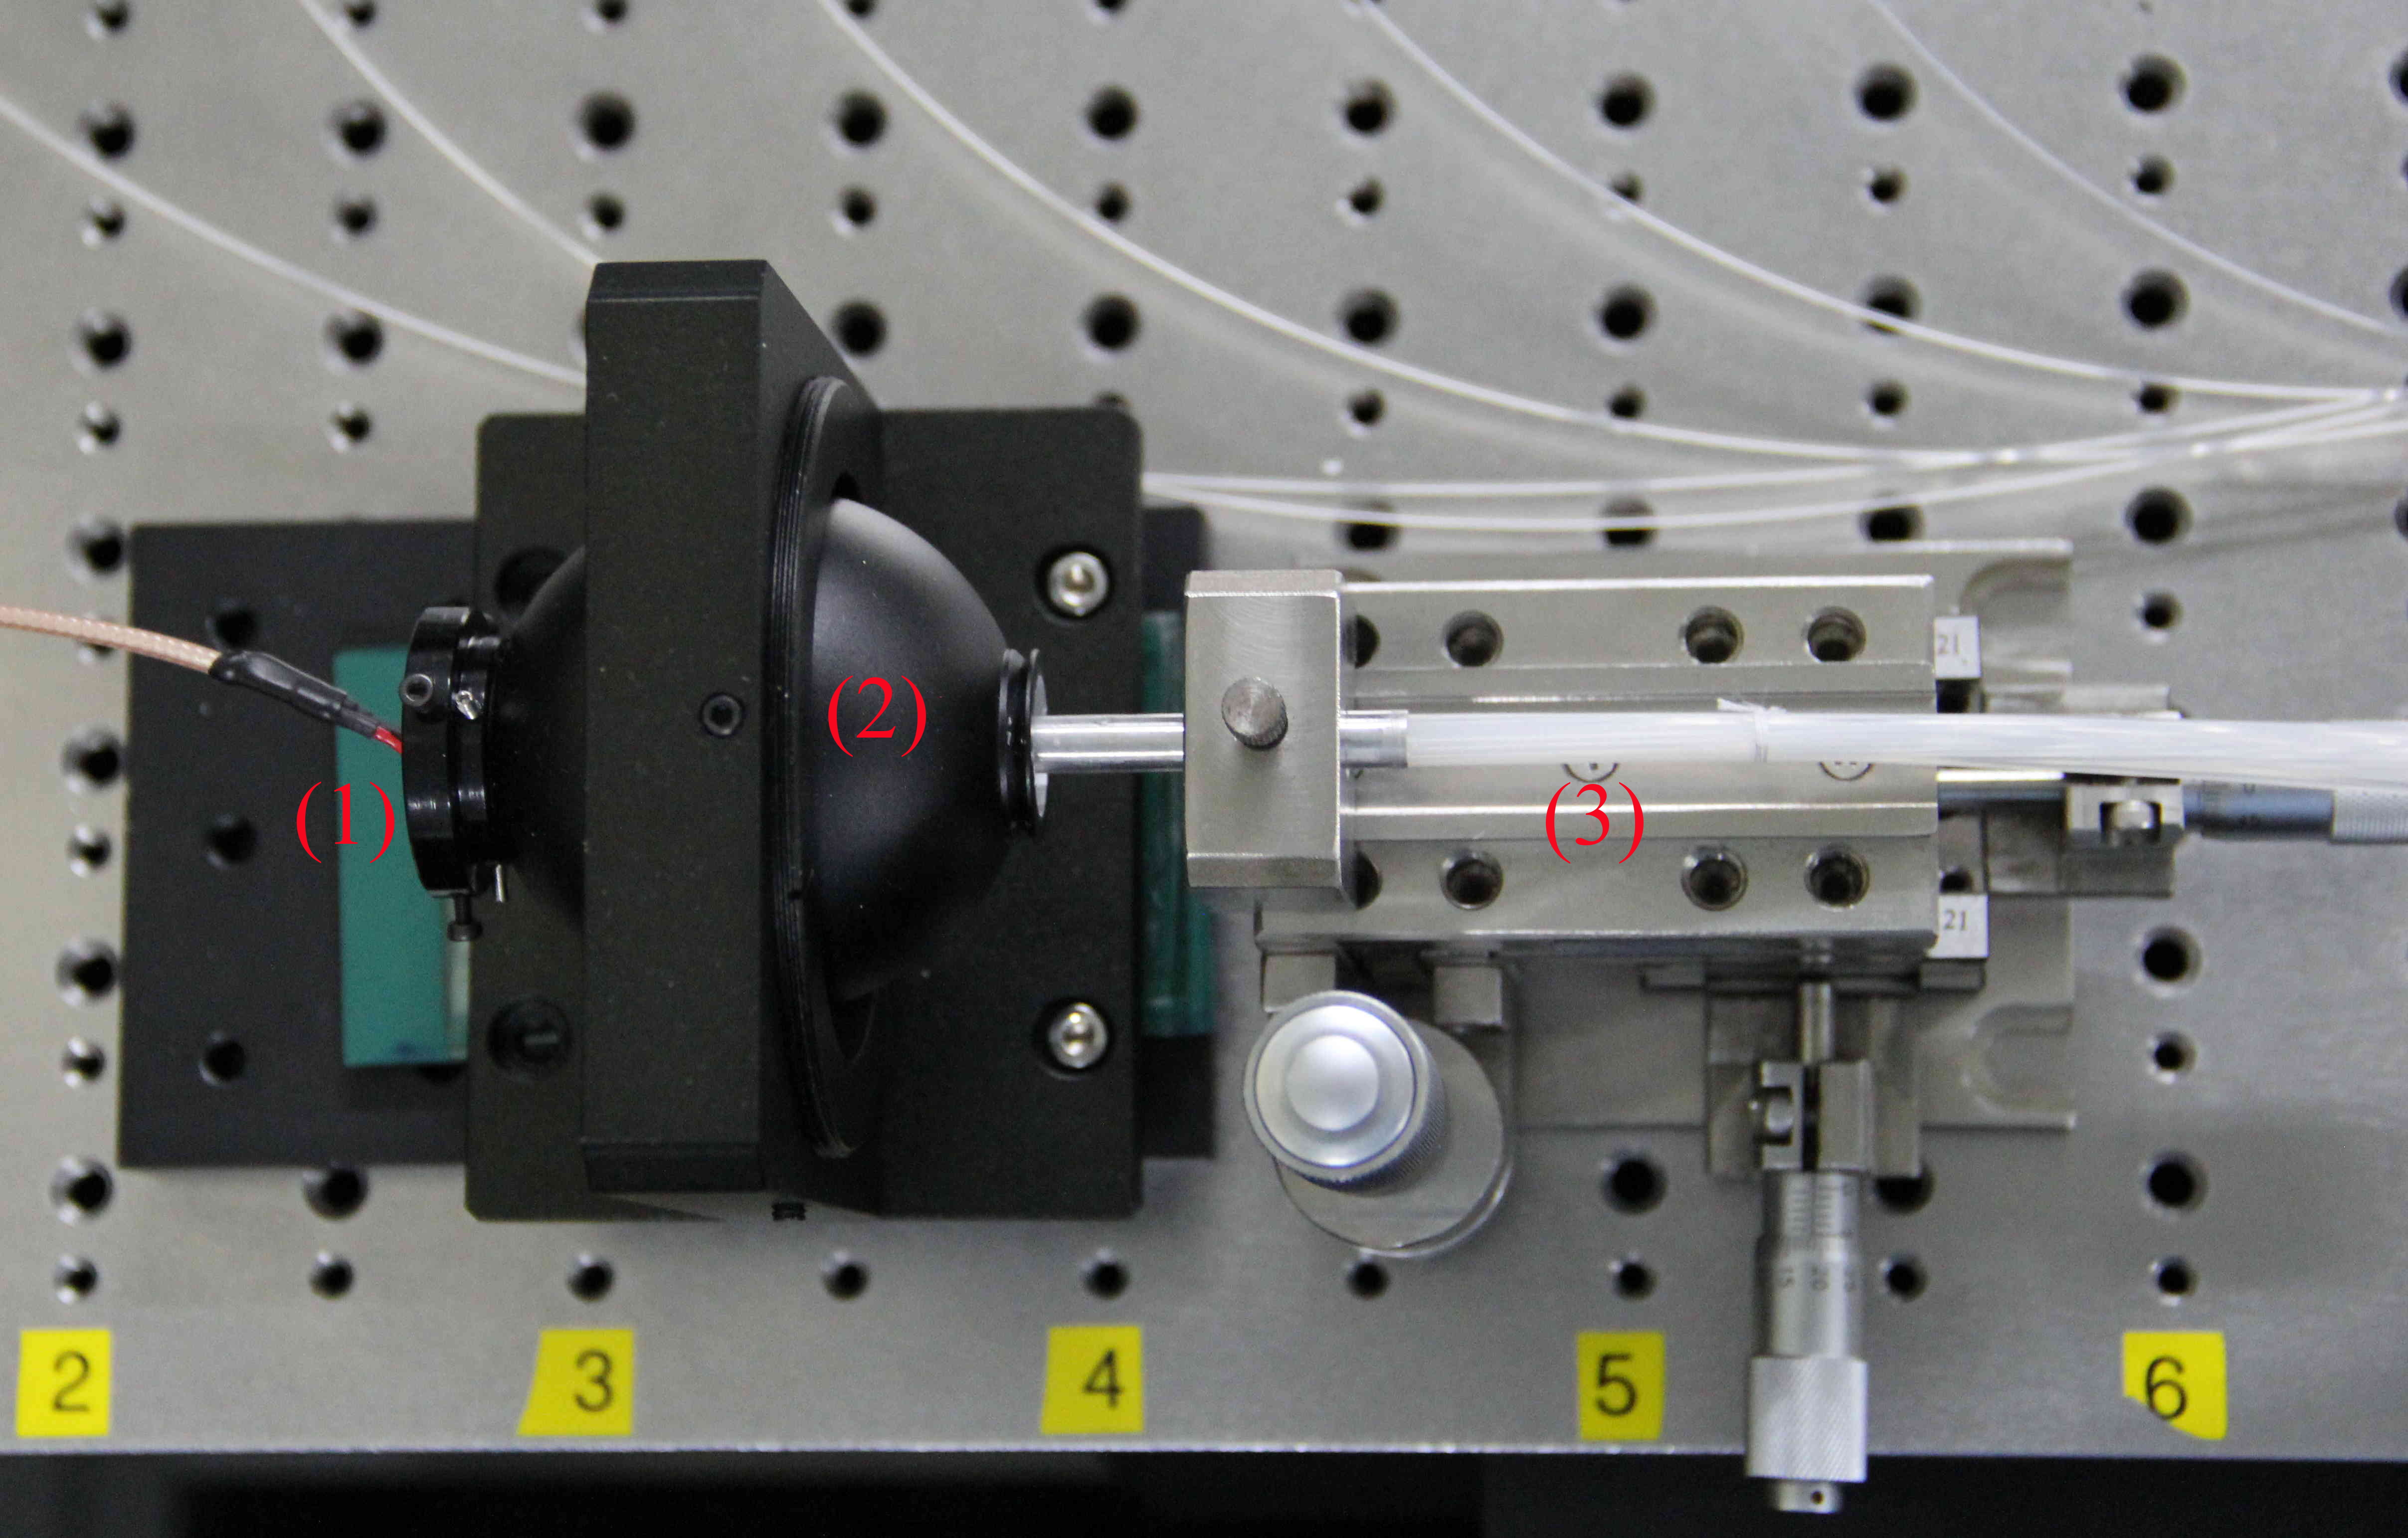
\includegraphics[width=90mm]{light_dist_label}
\caption{Integration of the light distribution system as a whole.
(1)LED glued on base (2)Integrating sphere (3)Fiber bundle}
\label{fig:light_source}
\end{figure} 

For easier manipulation and to protect the fibers from mechanical damage, both ends of the fiber bundle are coated with stainless steel ferrules.
The bundle end is coupled to the centre of the output port of integrating sphere using a stable fiber alignment stage.
On the other end, each fiber is fixed using a customized fiber holder which allows two-dimensional position adjustment and will be aligned to the centre of its corresponding PMT window with a precision of \SI{0.5}{\milli\meter}.

\begin{figure}
 \centering
 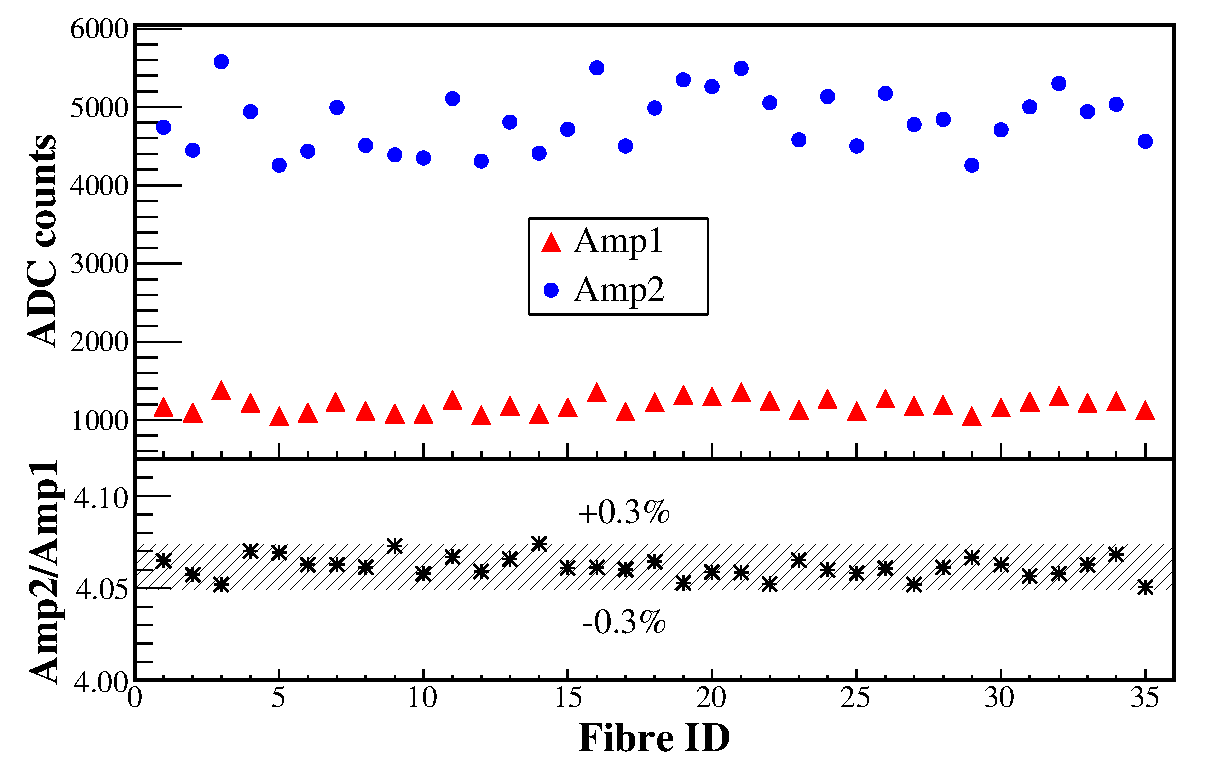
\includegraphics[width=90mm]{fibre_diff}
\caption{Up: Light output of different fibres measured at two light intensities of about 4 times difference.
Bottom: Ratio between the transmition difference measured at two light intesities, the results are consistent within \textpm\SI{0.3}{\percent}.}
\label{fig:fibre_diff}
\end{figure} 

The light output of each fiber was calibrated after coupling the bundle to the integrating sphere(see Fig.\ref{fig:light_source}).
For this calibration, the same PMT was used to scan all the fibers successively, while the light intensity fluctuation of the light source was monitored by another PMT.
After the light intensity correction, a variance of \SI{10}{\percent} is observed among the fibers as shown in Fig.\ref{fig:fibre_diff}, and this result is a direct reflection of the light transmition difference among the fibres because the contribution from light source non-uniformity is negligible.
Moreover, different light intensities were used in the calibration process, and the result shows that the transmition has no dependency on the light intensity used. 
This is whithin expectation, as the transmition coefficient is an intrinsic characteristic of the fiber itself.
The transmition difference of fibers from this calibration will be used as correction constants in the future measurements using this test bench.

\subsection{Software}
\label{sec:software}

As the PMT test bench is a combination of many different equipments and systems, an integrated control software will play a very important role. 
The software for the test bench is developped in Windows with C++ and divided into three hierarchies as follows:
\begin{enumerate}
 \item \textit{Device abstraction}, which not only serves as an interface to the underlying hardwares, but also handles the abstraction of different types of devices. 
 \item \textit{Framework libraries}, which defines a general testing pecedure and provides utility classes for configuration and management.
 \item \textit{User inerface}, which provides command line based or graphical executables for user interaction. 
\end{enumerate}

Instead of developping a dedicated program each time a hardware changes, an abstraction of the devices is adoptted to separate the testing procedure from hardware implementation details. 
Abstract classes are defined for the four essential types of controlling device as shown in the rounded boxes in Fig.\ref{fig:testbench_overveiw}.
New hardware only needs to inherit from the corresponding abstract class and implement its interface methods and then registered in the singlton class \textit{PTDeviceManager}, leaving all other part of the software unchanged.
Currently, concrete device classes for the hardware described in this section have all been implemented and fully tested.

Built upon the abstract device inerface, a general testing framework is defined as shown in Fig.\ref{fig:software_framework}.
\textit{PTVProgram} represents the measurement for a specific characteristic of PMT, such as cathode uniformity, gain and so on.
\textit{PTVTest} is a subunit of \textit{PTVProgram}, which encapsulates the real device operations performed under a specific condition.
A \textit{PTVProgram} may consist of a series of \textit{PTVTest}s, which are invoked sequentially in a test loop.
For example, in cathode uniformity measurement, the stepping motor will move to a series of positions and the PMT response will be recorded by the DAQ at each position.
Here, device operations performed at each position constitute a \textit{PTVTest} and tests at all positions constitute a \textit{PTVProgram}.
Additional operations may be added in the \textit{PreTest} and \textit{PostTest} methods of \textit{PTVProgram}, which will be invoked before and after the test loop repectively.
Typically, PMT warming can be performed in \textit{PreTest} and analysis can be done in \textit{PostTest}.
\textit{PTVProgram}s of various testing objectives will finally be chained together to constitute a complete characterization of PMT.

\begin{figure}
  \centering
 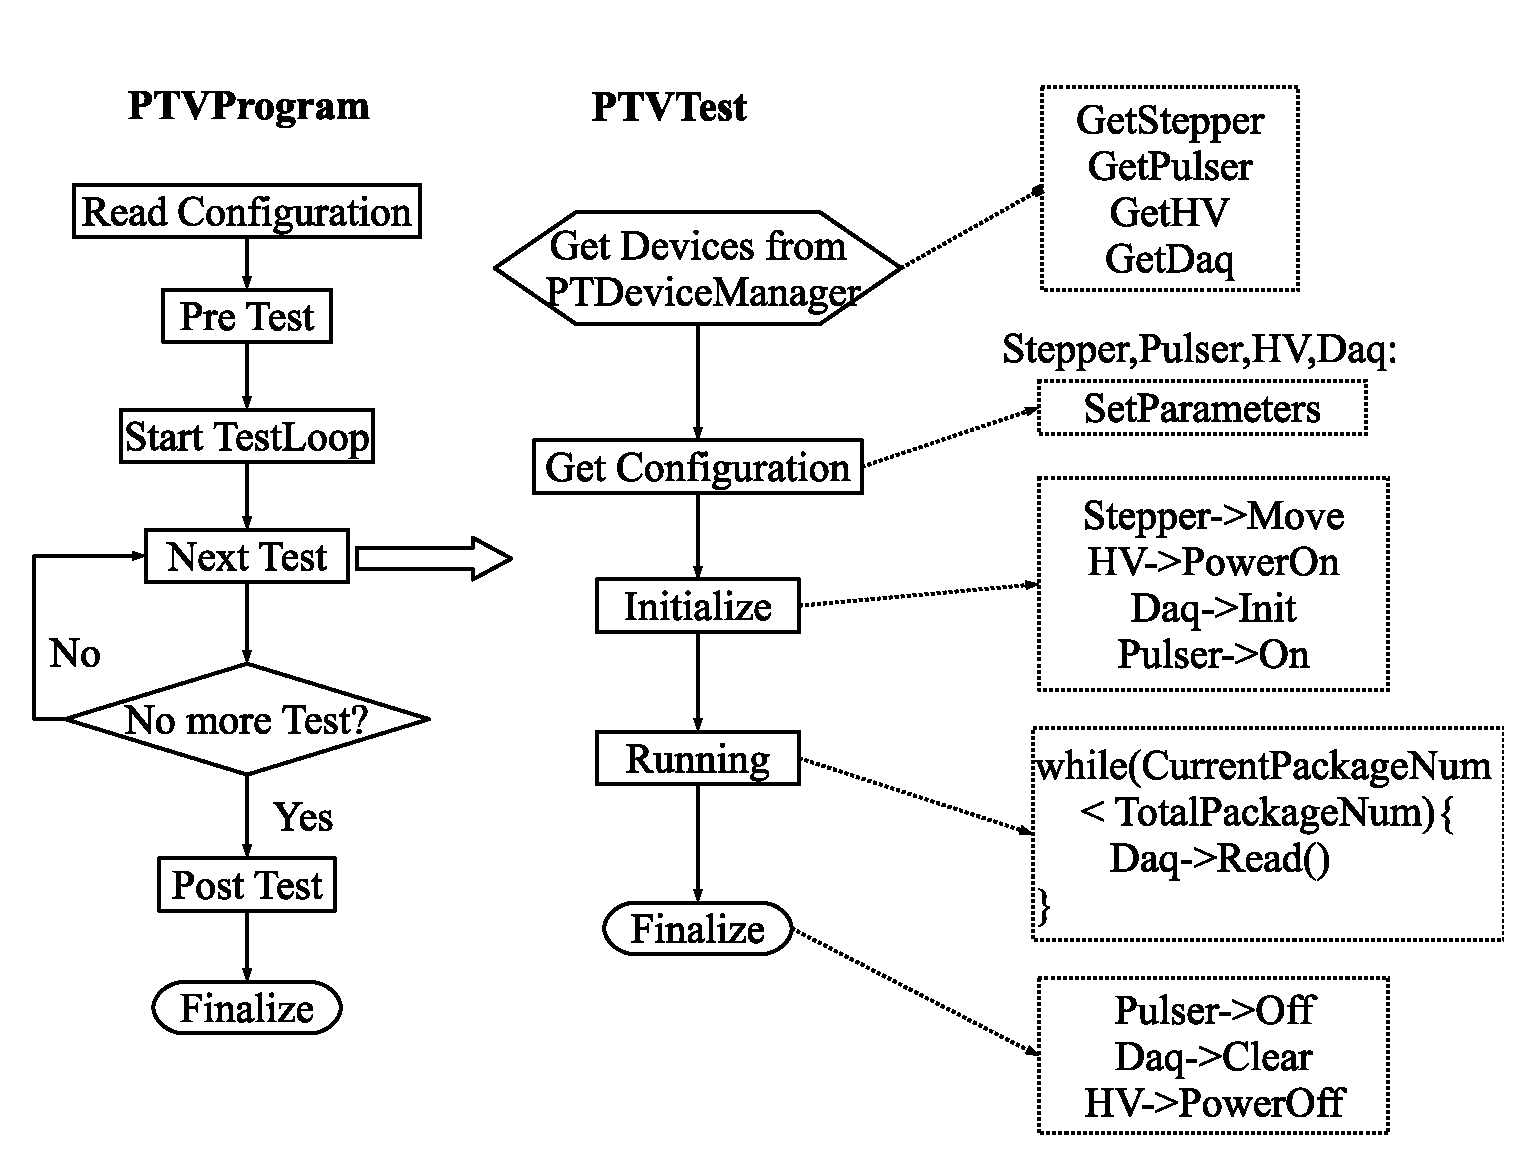
\includegraphics[width=140mm]{software_framework}
\caption{General PMT testing framework}
\label{fig:software_framework}
\end{figure}

For easy usage, a light-weight user interface based on PDCurses~\cite{pdcurses} has also been developped.
This program features in device control, status monitoring and information logging.
Thanks to the abstraction described above, the architecture of the program is rather independent of the specific hardware used and testing program performed.
A decoding function from binary file to root file~\cite{root} is also incorporated into it for online monitoring.
However, more detailed analysis are considered project specific and not included in the program. 

\section{Application in the construction of DAMPE PSD}
\label{sec:application}

\begin{figure}
 \centering
 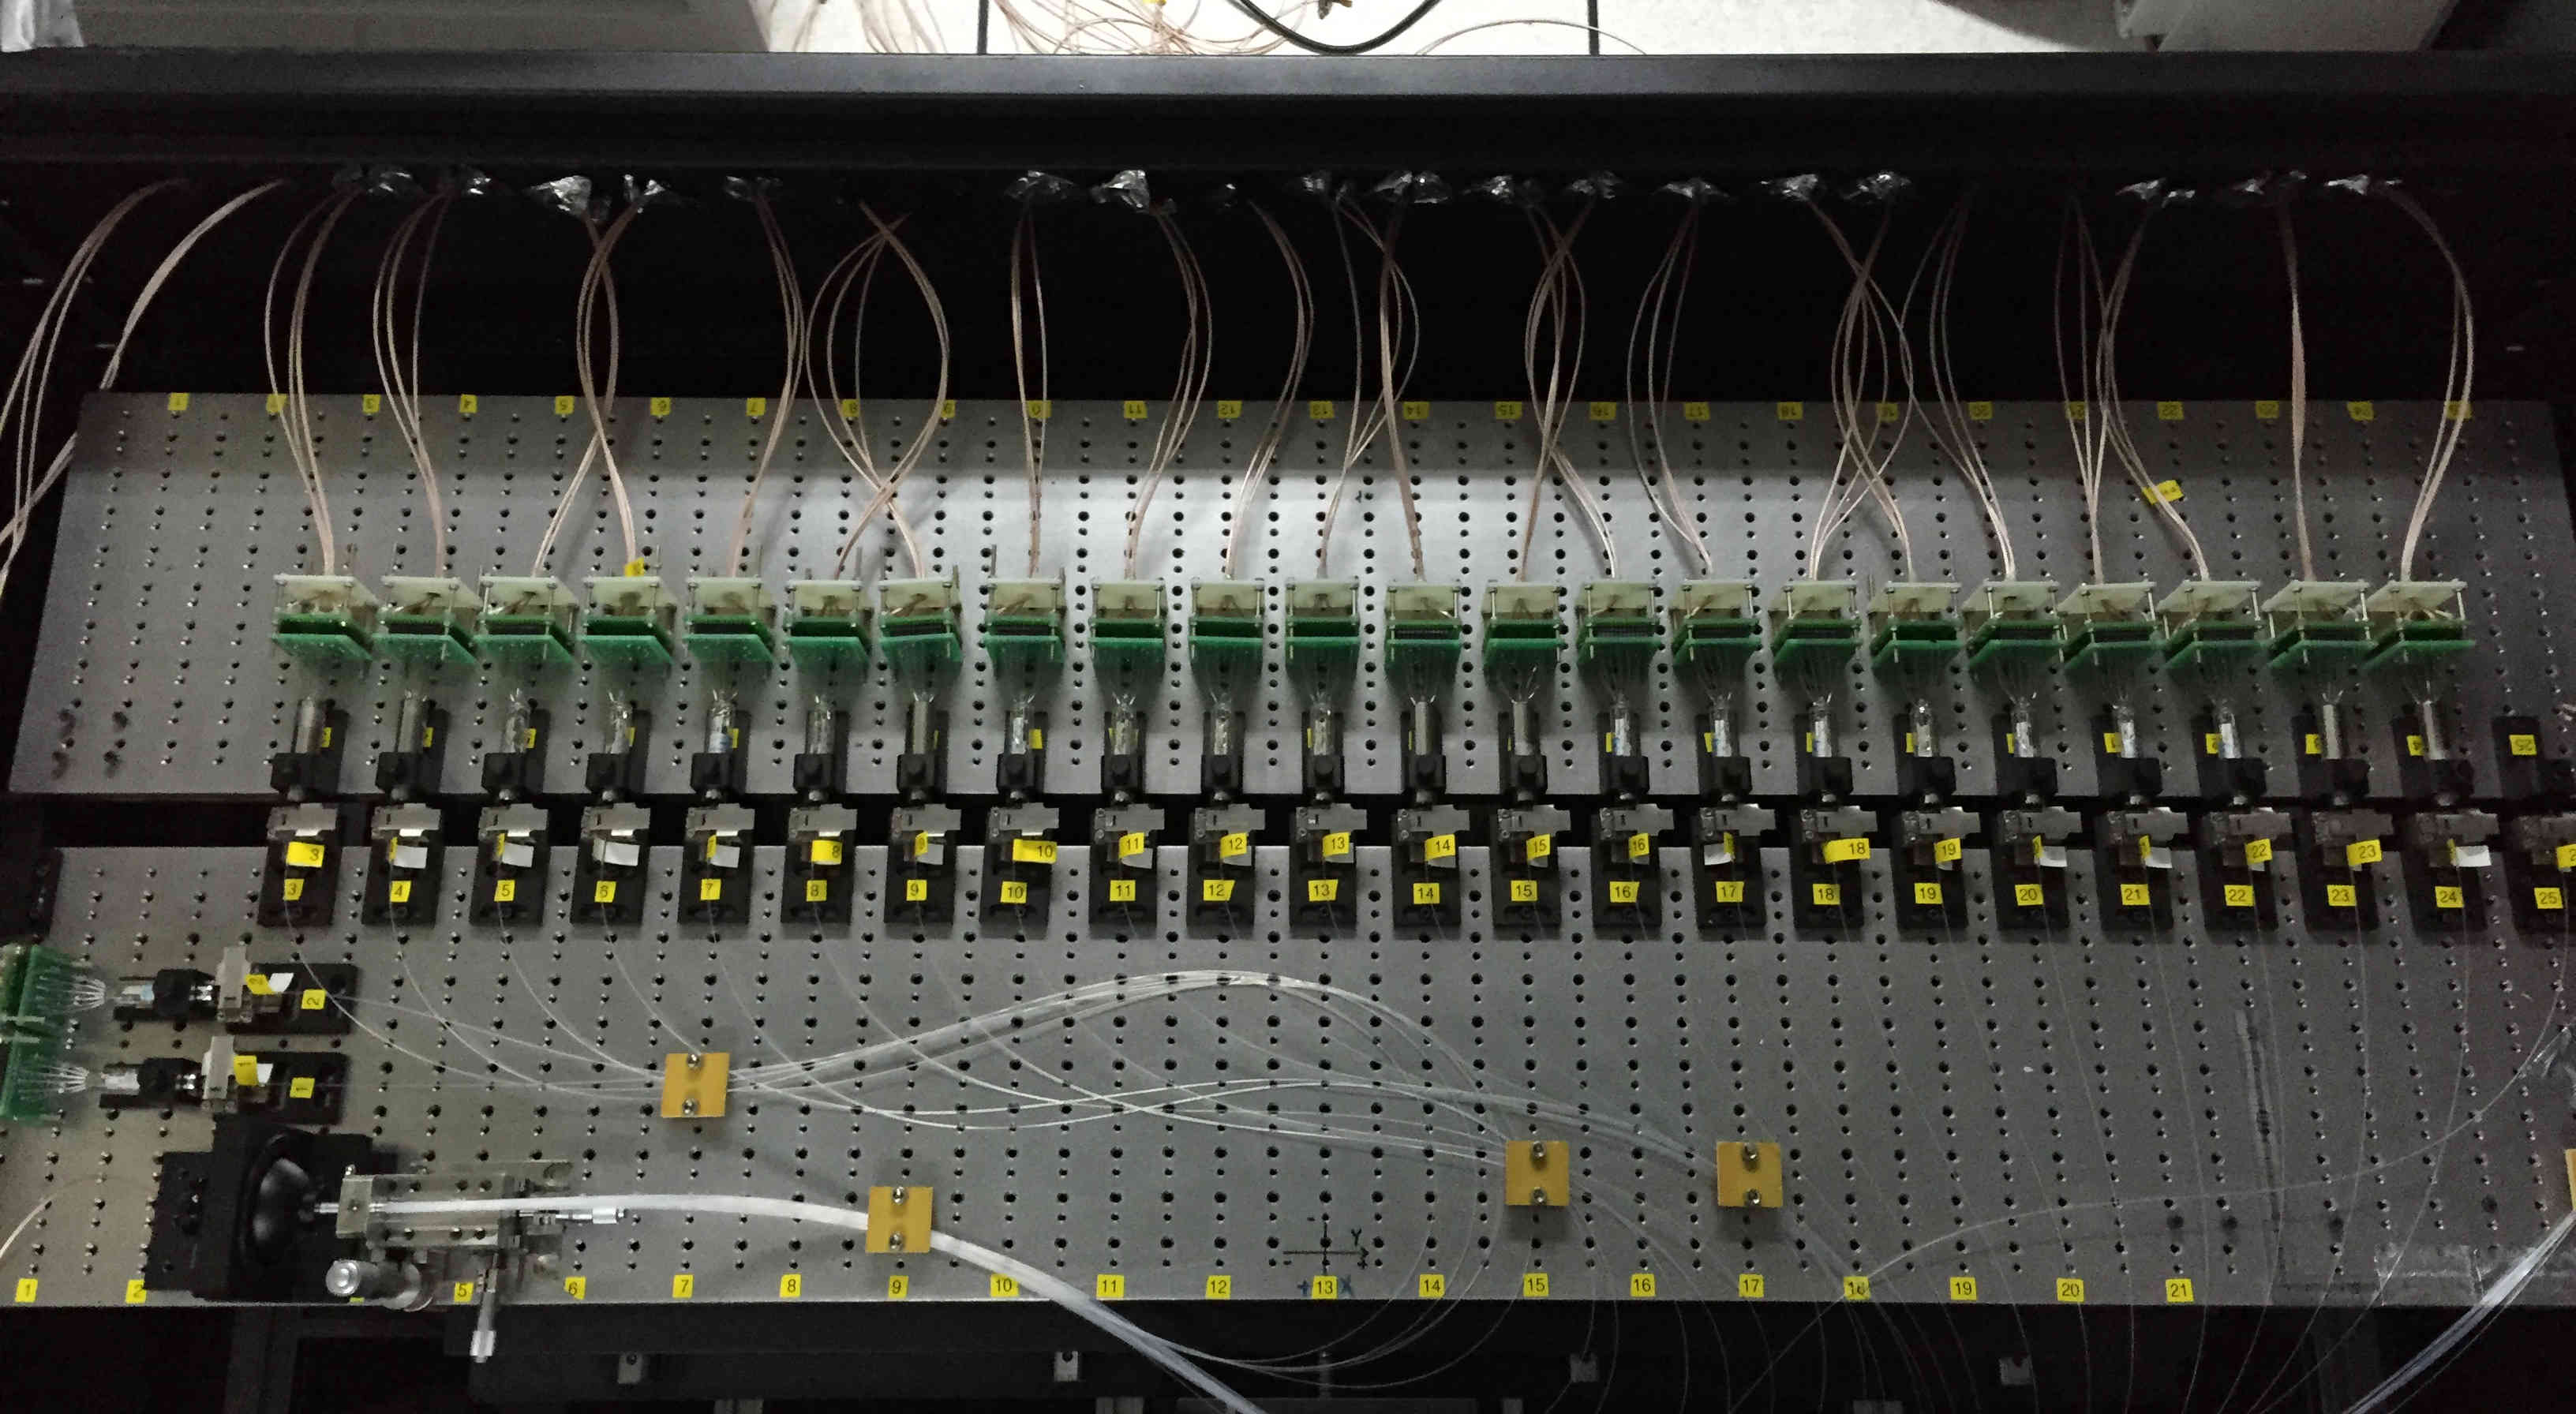
\includegraphics[width=140mm]{integration3}
\caption{Integration of all components of the test bench for R4443 Mod2 characterization.
Voltage dividers, same design as those used in the final assembly, are used. 
20 rare tubes are mounted and ready for test.
2 reference tubes can be seen in the bottom left corner of the picture. 
}
\label{fig:integrated_testbench}
\end{figure}

PSD adopts the Hamamastu R4443 PMT, which is ruggedized for space usage, for scintillation light detection. 
%R4443 is a \SI{14.5}{\milli\meter} 10 stages PMT with low noise bialkali photocathode.% and PSD will have 164 PMTs totally. 
To satisfy the large dynamic range requirement of PSD, two dynodes, 5 and 8, are readout for each PMT, and the signals are processed by a highly-sensitive ASIC chip(VA160~\cite{va160}) following with an ADC of 14~bits resolution~\cite{fee}. 
Besides the dynamic range, PSD also requires a \SI{25}{\percent} uniformity among all the PMTs(dynode8).% with certain HV applied. 
So both the gain of dynode8 and the gain between dynode8 and dynode5 of each PMT need to be measured before the installation.

Concrete \textit{PTVProgram}s for gain, dynode8/dynode5 ratio and cathode uniformity measurements have been implemented for this purpose.
To obtain more realistic results, a standalone data processing and acquiring system~\cite{fee} have been developped to replace the normal CAMAC system used with the PMT test bench. 
This new system is a clone of the real ones used in PSD and suitable for groud test of PSD components.
A dedicated \textit{PTVDaq} class based on NI-VISA library~\cite{ni_visa} has been implemented for it.

For a single run, about 20 tubes are mounted and tested, as shown in Fig.\ref{fig:integrated_testbench}, and it takes normally 5 hours, including 2 hour's PMT warming time. 
We performed 28 runs in a month, and totally 570 R4443 tubes have been studied carefully with this PMT test bench. 
All the data and analysis results are stored in a MySQL database for easy query, and the PMTs for PSD will be selected from these tubes.

Selection of tubes based the test data is not the object of this article.
Here, only the major results are presented with a focus on the demonstration of the validity of the test bench. 

\subsection{Gain of Dynode8}
\label{sec:psd_gain}

The gain of dynode8 is measured by recording the response of PMT at a certain setting of the light source. 
This is a relative method and the result depends on the light intensity:
\begin{equation}
 G_{relative} = L_i \times G(V) = L_i k V^\beta
 \label{equ:gain}
\end{equation}
where $G(V)$ is the absolute gain of PMT and $L_i$ is the light intensity at a specific light source setting.
$G_{relative}$ is a direct reflection of $G(V)$ if the inconsistency of light intensity can be eliminated between two measurements.
Two corrections are made to accomplish this goal, as follows: 
\begin{equation}
 G_{relative} = \frac{A_{Mean}}{K_{RunID} T_{ChID}}
 \label{equ:correction}
\end{equation} 
where $A_{Mean}$ is the mean value of the raw ADC spectrum at the specified light source setting,
$K_{RunID}$ is the light intensity fluctuation of LED between different test runs and $T_{ChID}$ is the light transmition difference among fibres of different testing channels.
$K_{RunID}$ can be calculated at each test run using the reference PMT.
$T_{ChID}$ is a constant parameter, which has been measured accurately before(Sec.\ref{sec:fiber_bundle}).
These corrections are made for all measurement results.

7 different high voltages, from \SIrange{700}{1000}{\volt} with a \SI{50}{\volt} step, are scanned to obtain the gain variation as a function of supply voltage for each PMT, and the results are fitted using the power law function.
Based on the fitting result,the relative gain at a certain supply voltage is calculated for comparison with the parameters on the data sheets provided by Hamamastu.
Linear correlation between the calculated gain and the anode blue sensitivity index has been observed, while no relation to the cathode blue sensitivity has been found(see Fig.\ref{fig:gain_correlation}).
This result is a direct demonstration of the validity of our testing method.

5 light source settings, with a maximum intensity difference of about 2 times, have been used for relative gain measurement.
The results from different light intensities are cross checked and they are consistent with each other.
Distribution of the relative gain at 850V is shown in Fig.\ref{fig:gain_dist}, where all the tubes are normalized to the one with the smallest gain. 
A maximum of about 6 times difference in the gain has been observed.

\begin{figure}
 \centering
 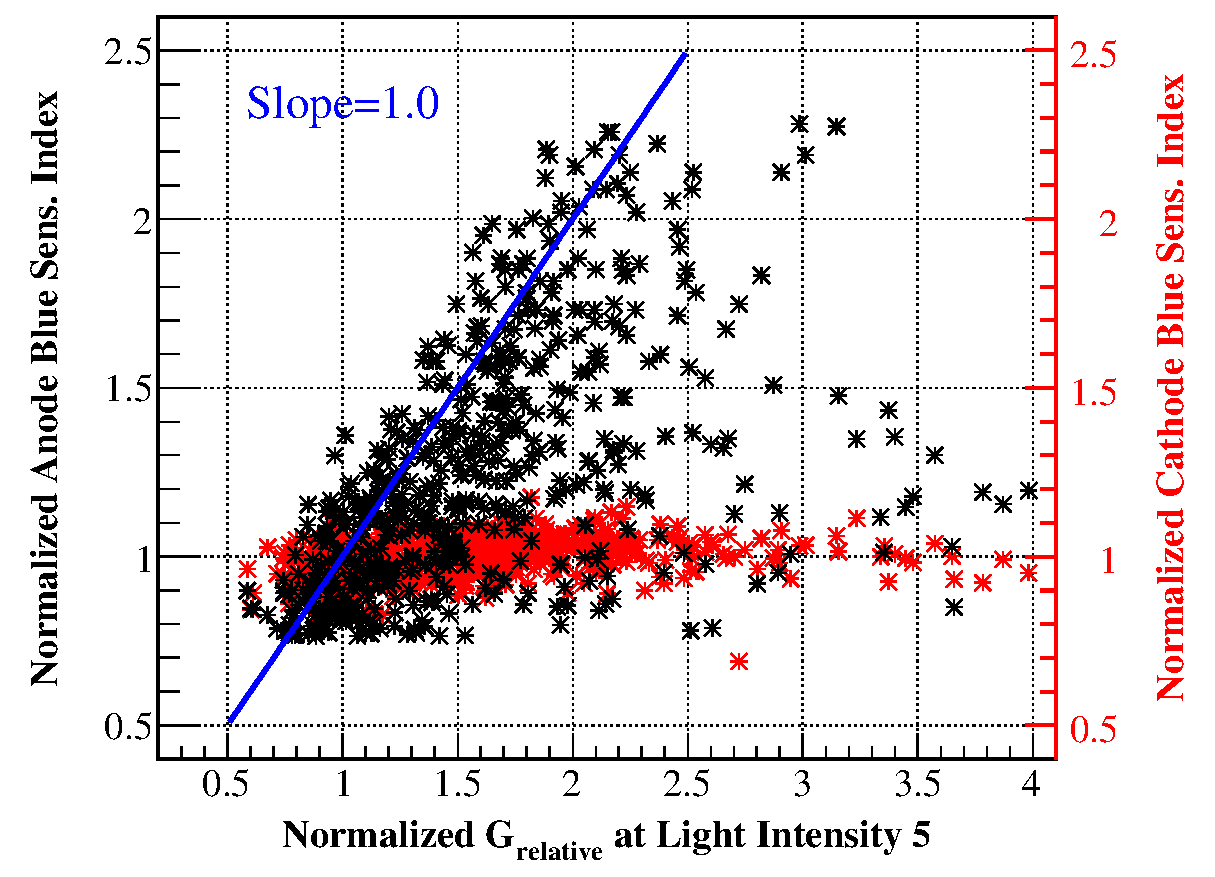
\includegraphics[width=90mm]{correlation_new}
\caption{Correlation between the parameters given by Hamamastu and the gain measured using the test bench.
Data are normalized to the same tube.}
\label{fig:gain_correlation}
\end{figure} 

\begin{figure}
 \centering
 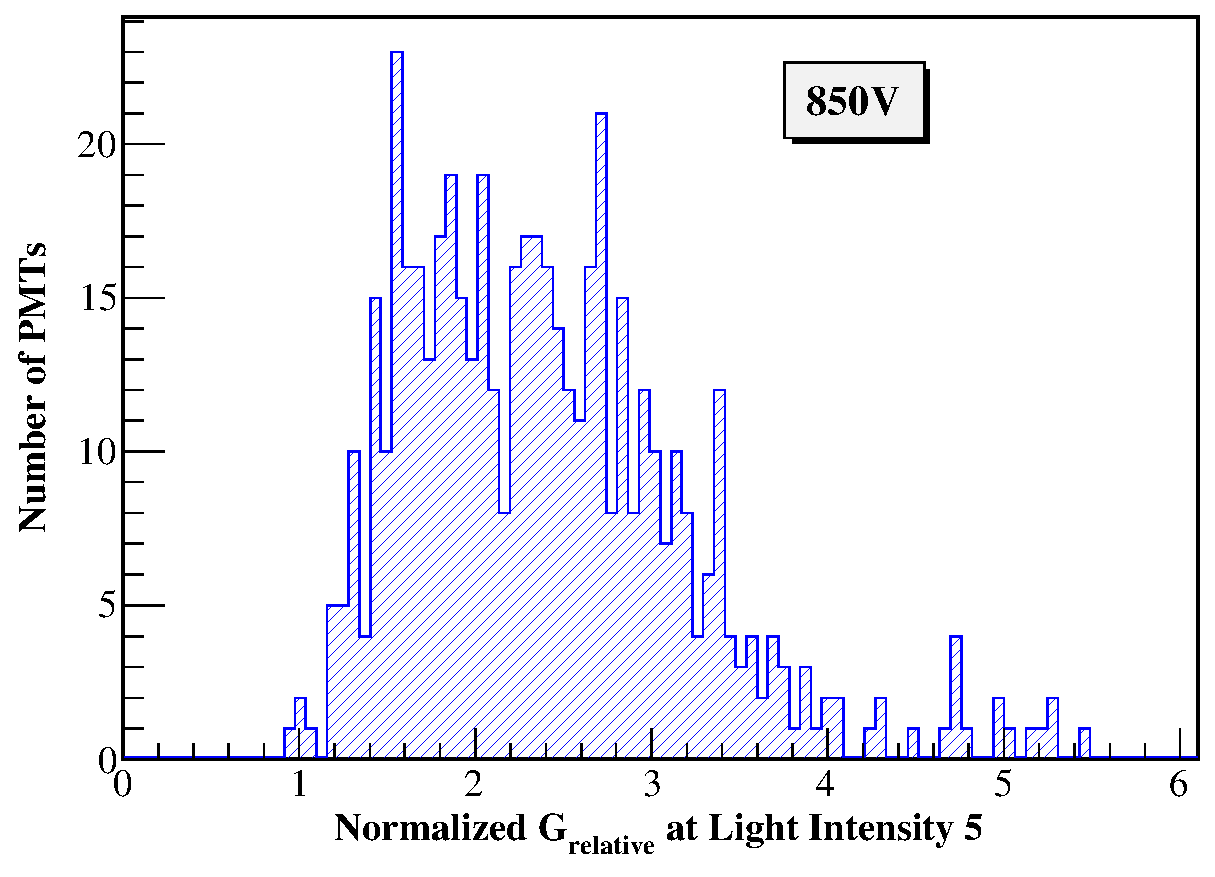
\includegraphics[width=90mm]{GainDist}
\caption{Relative gain distribution at 850V measured using light intensity 5.
Data are normalized to a specific tube of small gain.}
\label{fig:gain_dist}
\end{figure}

\subsection{Gain ratio between Dynode8 and Dynode5}
\label{sec:psd_dy58}

\begin{figure}
 \centering
 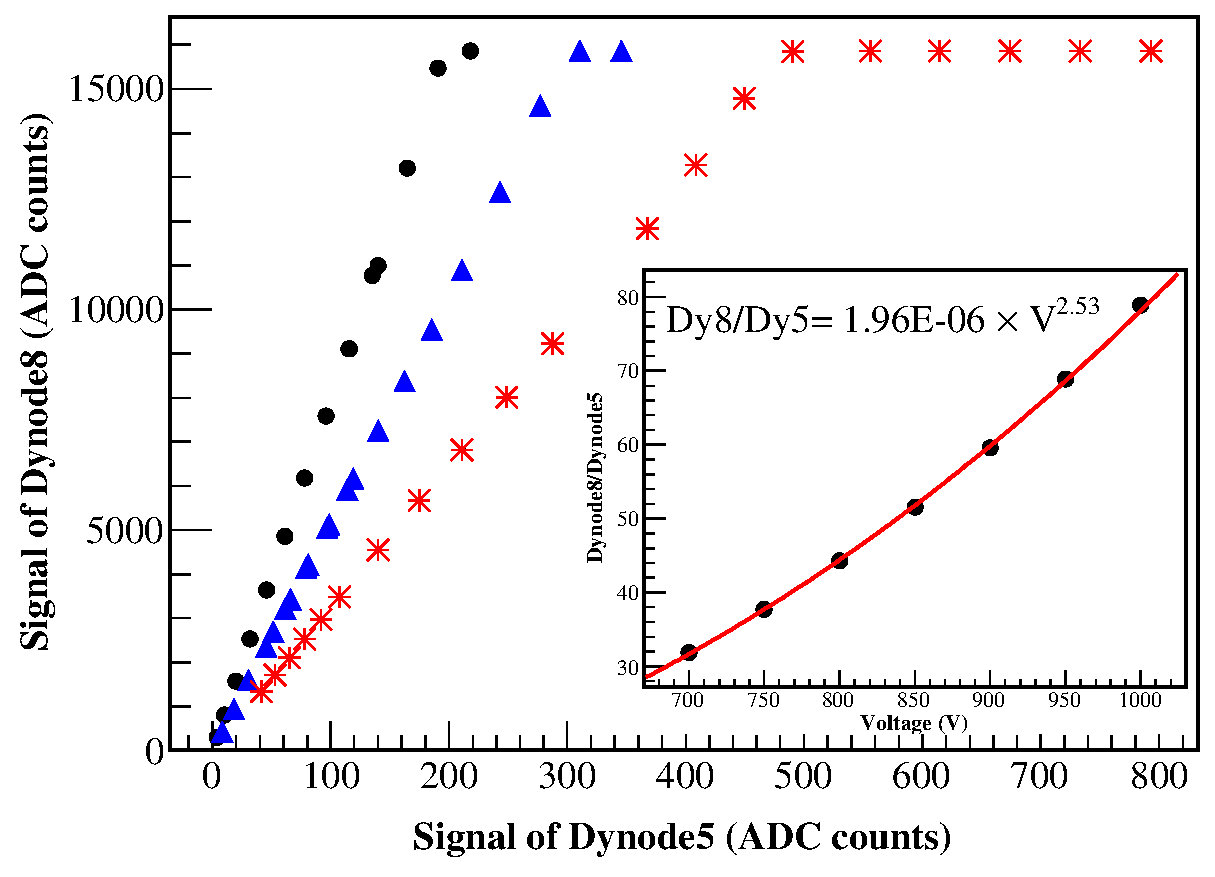
\includegraphics[width=90mm]{dy58_example}
\caption{Example of the measurement of dynode8/dynode5.
Correlation between dynode5 and dynode8 at 1000V, 850V and 700V is presented for a typical tube.
Power law fit to the measured dynode8/dynode5 at 7 voltage steps is shown in the inset graph.
}
\label{fig:dy58_example}
\end{figure} 

The gain ratio between dynode8 and dynode5 is measured by varying the light intensity in a large range until saturation of the dynode8 singal is observed, as shown in Fig\ref{fig:dy58_example}.
The same procedure is repeated at 7 different supply voltages, from \SIrange{700}{1000}{\volt} with a \SI{50}{\volt} step, to obtain the dynode8/dynode5 dependency on voltage.
As with the gain of dynode8, the dependency can be fitted accurately with a power law function, as shown in the inset graph of Fig.\ref{fig:dy58_example}.
The ratio between the gain of dynode8 and dynode5 can then be calculated at any voltage value based on the fitting result.
As an example, the distribution of dynode8/dynode5 ratios at a centain supply voltage is shown in Fig.\ref{fig:dy58_dist}.
It can been seen that the variance is much smaller than that of gain.

\begin{figure}
 \centering
 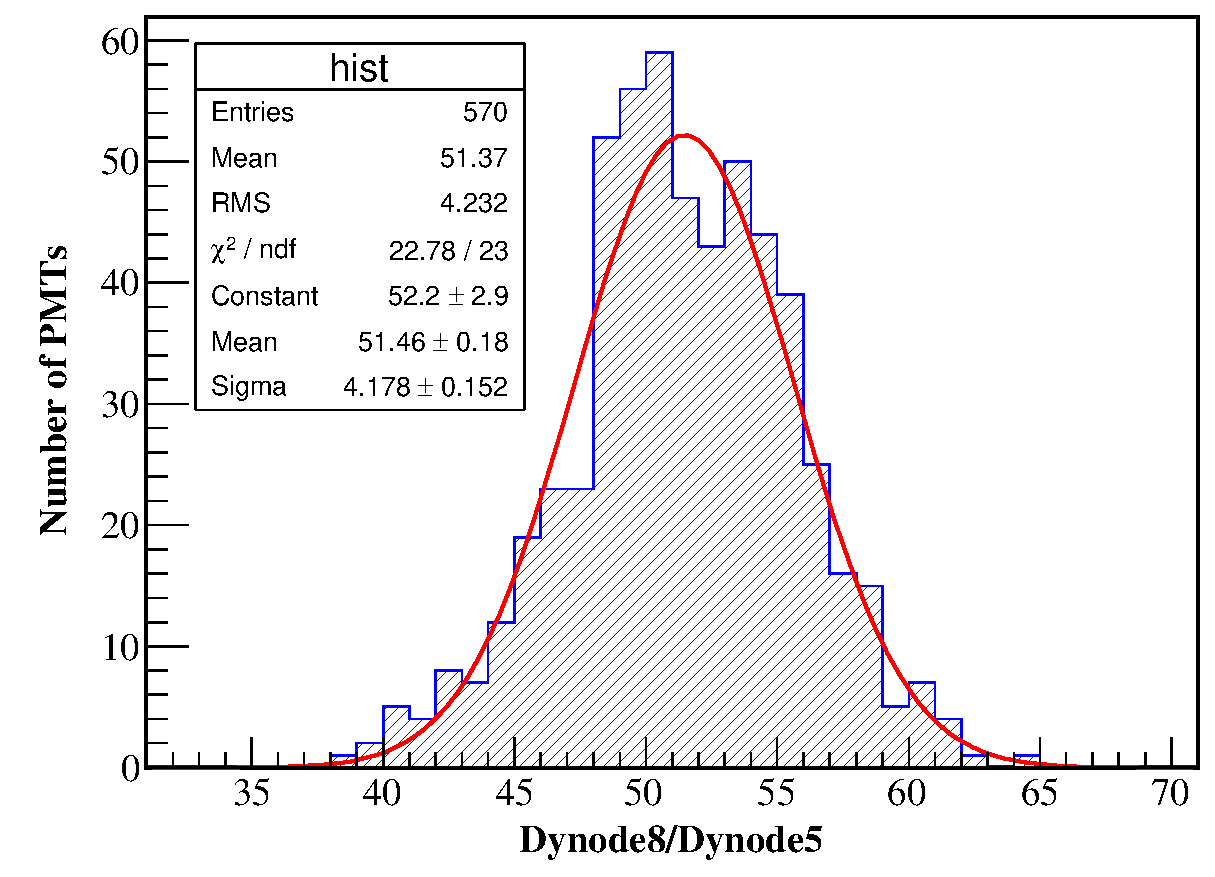
\includegraphics[width=90mm]{dy58_dist}
\caption{Distribution of the Dynode8/Dynode5 at the Hamamastu equivalent voltage.}
\label{fig:dy58_dist}
\end{figure} 

\subsection{Cathode Uniformity}
\label{sec:psd_cathodescan}

\begin{figure}
 \centering
 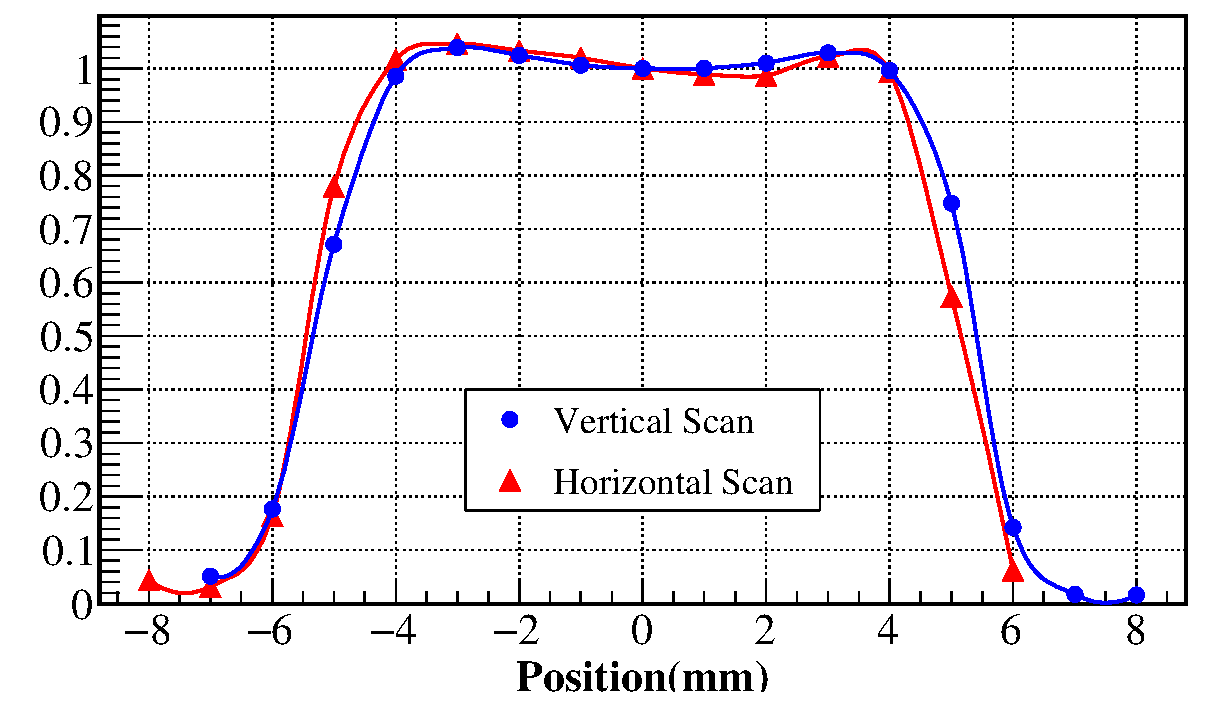
\includegraphics[width=90mm]{cathode_uniformity}
\caption{A typical cathode uniformity of R4443.
Relative gain at each position is normalized to the center of the input window.}
\label{fig:cathode_uniformity}
\end{figure} 

R4443 has a photocathode with a minimum effective area of about \SI{10}{\milli\meter} in diameter, and the uniformity of the cathode can also be checked using our test bench.
This measurement is done by scanning the input window of R4443 with a step of \SI{1}{\milli\meter} in two directions that are perpendicular to each other.
At each position, the relative gain is measured at a fixed light source setting according to the method described in Sec.\ref{sec:psd_gain}, and a typical result is shown in Fig.\ref{fig:cathode_uniformity}.

The relative gain we measured at each position is proportional to the total efficiency of light transmission, photoelectric conversion and electron collection at this point, and we can see the rapid drop of this efficiency at the edge of the cathode surface. 
If we define the uniform region as a region with the efficiency fluctuation less than \SI{10}{\percent}, we found that only \SI{75}{\percent} of the tested PMTs can have a uniform region larger than \SI{9}{\milli\meter} in diameter. 

\section{Summary}
\label{sec:summary}

A PMT test bench has been developped at IMP, CAS. 
It's suitable for massive PMT test and has been applied in the construction of DAMPE PSD already.
Because the PMT test bench is monitored by two reference PMTs all the time, we can also get some knowledge about the performance of this system using the data obtained in the PMT characterization for DAMPE PSD.

The stability of these reference PMTs is checked firstly.
The ratio, $M$, between the response of two reference PMTs is a parameter irrelevant to the light intensity: 
\begin{equation}
 M = \frac{G_{ref1} T_{ref1}}{G_{ref2} T_{ref2}}
 \label{equ:stability}
\end{equation}
where $G_{ref}$ is the absolute gain of the reference PMT and $T_{ref}$ is the transmition coefficient of fibers coupled to this reference channel.
As $T_{ref}$ is a constant parameter, $M$ is only related to the gain difference between the reference PMTs.
Because these two PMTs are completely independent, $M$ is a good candidate to monitor the stability of the two PMTs. 
We checked the $M$ values from all test runs, and only found a small variance of \SI{0.48}{\percent}. 

By checking the response of these reference PMTs to a certain setting of the light source, a maximum variation of \SI{4}{\percent} in the light intensity of LED is observed during a period of about one month.
Light intensity fluctuation can be corrected using the method described in \ref{sec:psd_gain}.
As two reference PMTs exists, this method can be validated by using one of them for correction and then checking the relative gain of the other. 
The result is shown in Fig.\ref{fig:led_stability}.
After the correction, stability of the light source is controlled within \textpm\SI{0.5}{\percent}.

\begin{figure}
 \centering
 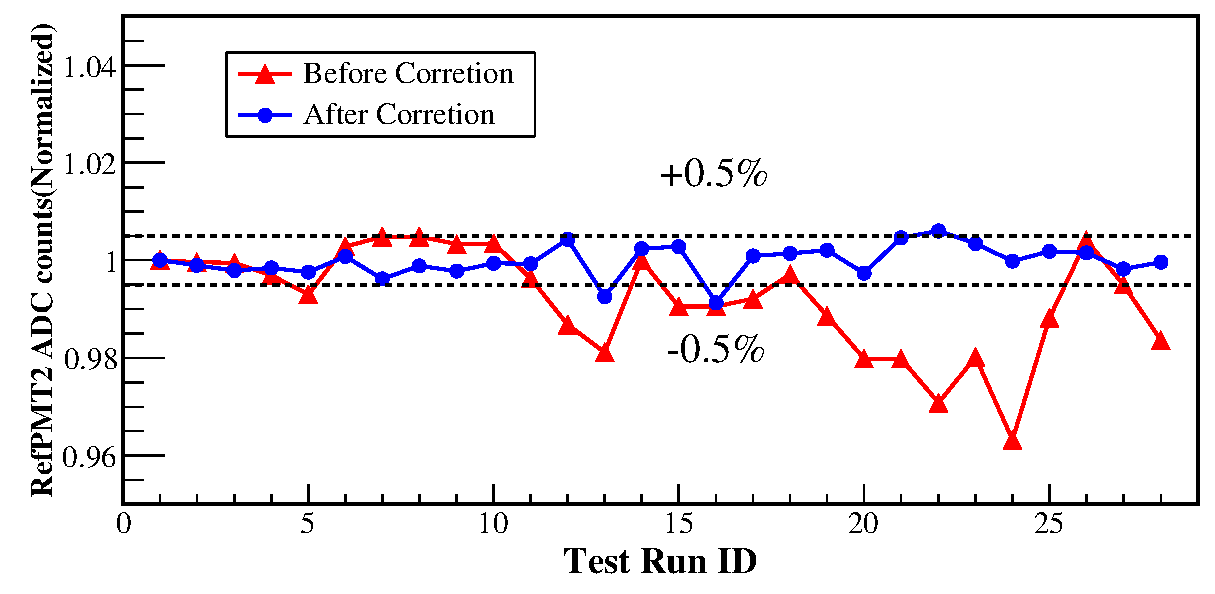
\includegraphics[width=80mm]{led_stability}
\caption{Stability of the light source monitored by Reference PMT2 at 900V.
The data corresponds to a period of about one month and is all scaled to the first test run.
Red line: mean value of raw ADC counts, recorded at the same light source setting before light intensity correction.
Blue line: relative gain, measured after using Reference PMT1 for light intensity correction.}
\label{fig:led_stability}
\end{figure} 

Reference PMTs underwent the same testing procedures as the tubes under test.
Thus, spread of the distribution of parameters of the reference PMTs is an indication of the uncertainty of the testing method.
As an example, distribution of the ratio between dynode8 and dynode5 of the reference PMTs is shown in Fig.\ref{fig:dy58_stabiltiy}, where the results from different voltage steps are normalized to their respective mean value of all test runs and filled together.
The variance is \SI{1.59}{\percent}, which is adoptted as the testing uncertainty of the dynode8/dynode5 measurement.
In the same way, the uncertainty in the measurement of relative gain is estimated to be \SI{0.53}{\percent}. 

\begin{figure}
 \centering
 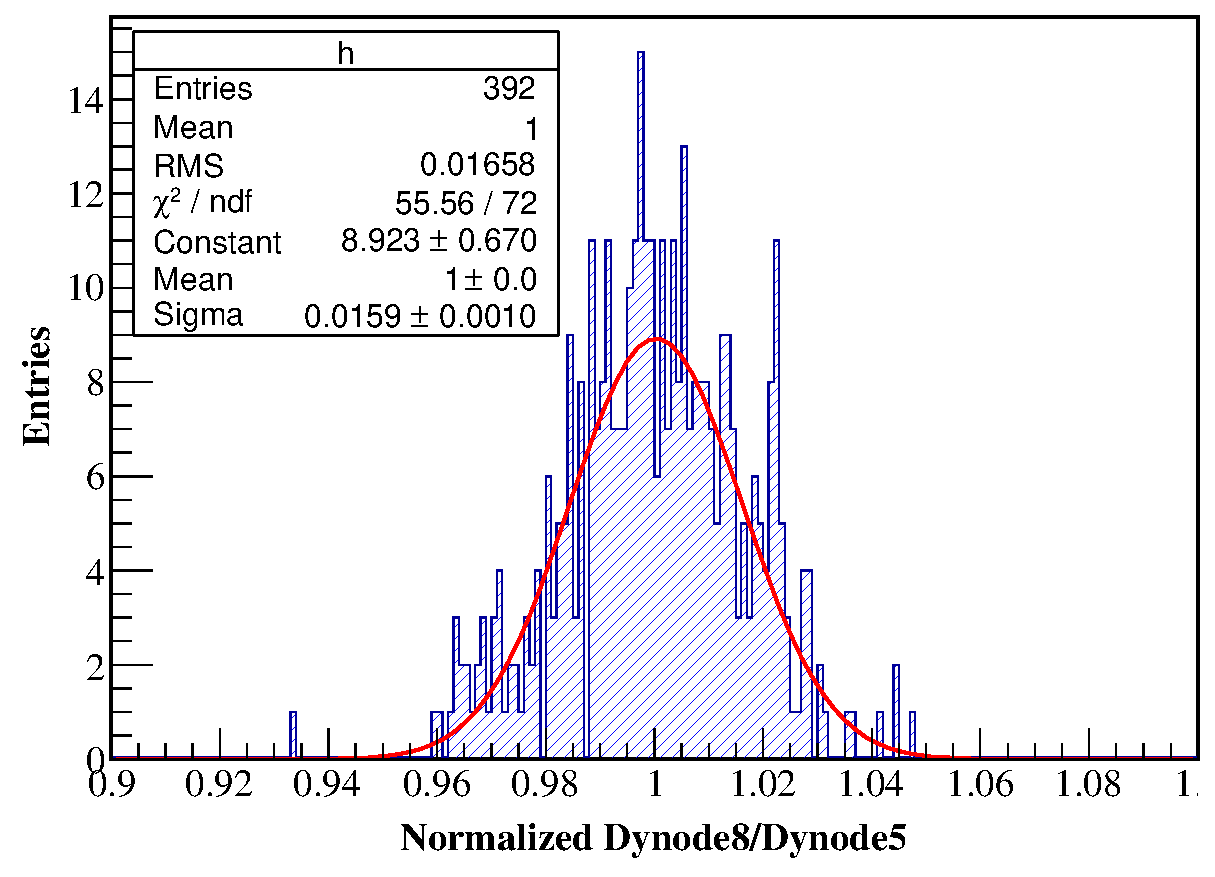
\includegraphics[width=80mm]{RefDy58Dist}
\caption{Distribution of the ration between dynode8 and dynode5 of the reference PMTs measured by the test bench.
Results from all voltage steps are normalized to their respective mean value of all test runs.}
\label{fig:dy58_stabiltiy}
\end{figure} 

All these results have proved the high reliablity of our test bench system.
Considering the flexible and open platform it possesses, the test bench is also useful for any other projects that need massive PMT characterization. 

%%%%%%%%%%%%%%%% Acknowledgement %%%%%%%%%%%%%%%%%%%%%%%
\section*{Acknowledgement}

This work was supported by the Strategic Priority Research Program of the Chinese Academy of Science under Grant No. XDA04040202-3.

%%%%%%%%%%%%%%%%    Appendix     %%%%%%%%%%%%%%%%%%%%%%%
%% The Appendices part is started with the command \appendix;
%% appendix sections are then done as normal sections
%\appendix
%\section{}
%\label{app:}

%%%%%%%%%%%%%%%%   Bibliography  %%%%%%%%%%%%%%%%%%%%%%%
%% bibliography style
\section*{References}
\bibliographystyle{elsarticle-num}

%% From BibTex file
\bibliography{mybib}

%% From hand-writing
\begin{comment}
%%\begin{thebibliography}{00}

%%\bibitem{CEBAF12}
%%V.D. Burkert,  \emph{arXiv:1203.2373v1 [nucl-ex]},  2012.

%%\bibitem{CLAS}
%%B.A. Mecking \emph{et al.},  Nucl. Ins. and Meth. in Phys. Research {\bf A503} (2003) 513

%%\end{thebibliography}
\end{comment}

\end{document}
\endinput